\documentclass[tikz,border=3pt]{standalone}
\usepackage{amsmath}
\usetikzlibrary{arrows.meta,positioning,calc,fit}
\newcommand{\Cuk}{\mbox{\'{C}uk}}
\definecolor{esrblue}{RGB}{34,91,151}
\definecolor{caporange}{RGB}{190,92,20}
\definecolor{gategray}{RGB}{90,96,105}
\definecolor{superviolet}{RGB}{115,46,153}
\begin{document}
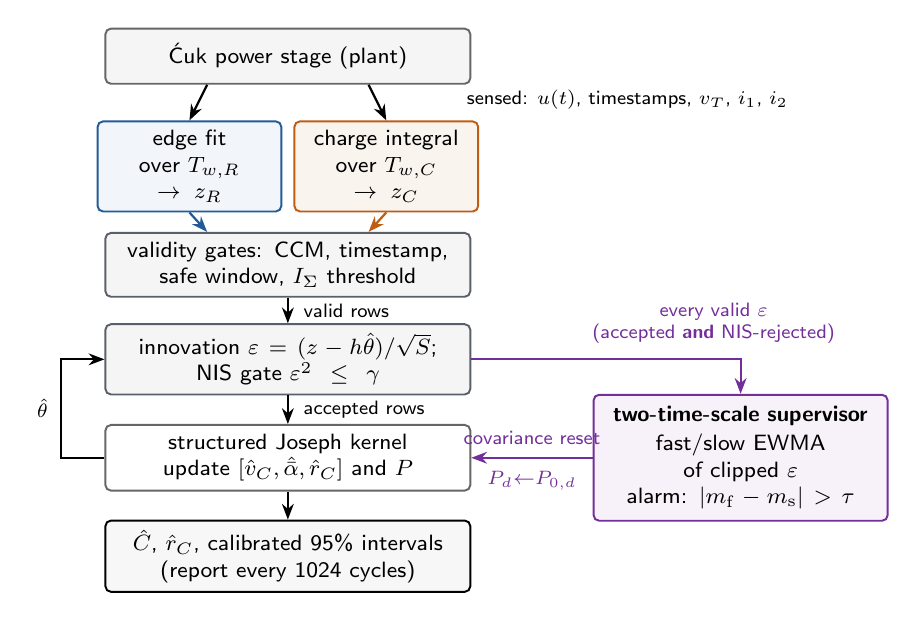
\begin{tikzpicture}[
  font=\sffamily\footnotesize,
  block/.style={rounded corners=2pt,draw=black!60,fill=white,align=center,
    minimum height=7mm,line width=0.7pt},
  esr/.style={block,draw=esrblue,fill=esrblue!6},
  cpath/.style={block,draw=caporange,fill=caporange!7},
  sup/.style={block,draw=superviolet,fill=superviolet!6},
  arr/.style={-{Stealth[length=2.0mm]},line width=0.8pt},
  suparr/.style={arr,draw=superviolet},
  lbl/.style={font=\sffamily\scriptsize}]

\node[block,fill=black!4,text width=44mm] (plant) at (2.6,6.60)
  {\Cuk{} power stage (plant)};
\node[esr,text width=21mm,minimum height=9mm] (efit) at (1.35,5.20)
  {edge fit over $T_{w,R}$\\$\to z_R$};
\node[cpath,text width=21mm,minimum height=9mm] (cint) at (3.85,5.20)
  {charge integral over $T_{w,C}$\\$\to z_C$};
\node[block,draw=gategray,fill=black!4,text width=44mm] (vgate) at (2.6,3.95)
  {validity gates: CCM, timestamp,\\
   safe window, $I_\Sigma$ threshold};
\node[block,draw=gategray,fill=black!4,text width=44mm] (innov) at (2.6,2.75)
  {innovation $\varepsilon=(z-h\hat\theta)/\sqrt{S}$;\\
   NIS gate $\varepsilon^{2}\le\gamma$};
\node[block,text width=44mm] (kern) at (2.6,1.50)
  {structured Joseph kernel\\update $[\hat v_C,\hat{\bar\alpha},\hat r_C]$
   and $P$};
\node[block,draw=black,fill=black!3,text width=44mm] (outp) at (2.6,0.25)
  {$\hat C$, $\hat r_C$, calibrated 95\% intervals\\
   (report every 1024 cycles)};
\node[sup,text width=35mm,minimum height=16mm] (supv) at (8.35,1.50)
  {\textbf{two-time-scale supervisor}\\[1pt]
   fast/slow EWMA of clipped $\varepsilon$\\
   alarm: $|m_{\mathrm f}-m_{\mathrm s}|>\tau$};

\draw[arr] ($(plant.south west)!0.28!(plant.south east)$) -- (efit.north);
\draw[arr] ($(plant.south west)!0.72!(plant.south east)$) -- (cint.north);
\node[lbl,anchor=west] at (4.75,6.05)
  {sensed: $u(t)$, timestamps, $v_T$, $i_1$, $i_2$};
\draw[arr,esrblue] (efit.south) --
  ($(vgate.north west)!0.28!(vgate.north east)$);
\draw[arr,caporange] (cint.south) --
  ($(vgate.north west)!0.72!(vgate.north east)$);
\draw[arr] (vgate.south) -- (innov.north)
  node[lbl,midway,right=2pt] {valid rows};
\draw[arr] (innov.south) -- (kern.north)
  node[lbl,midway,right=2pt] {accepted rows};
\draw[arr] (kern.south) -- (outp.north);
% estimate feedback into the innovation
\draw[arr] (kern.west) -- ++(-0.55,0) |- (innov.west)
  node[lbl,pos=0.25,left=1pt] {$\hat\theta$};
% supervisor tap and reset
\draw[suparr] (innov.east) -| (supv.north)
  node[lbl,pos=0.45,above=2pt,superviolet,align=center]
  {every valid $\varepsilon$\\(accepted \textbf{and} NIS-rejected)};
\draw[suparr] (supv.west) -- (kern.east)
  node[lbl,midway,above=1pt,superviolet] {covariance reset}
  node[lbl,midway,below=1pt,superviolet] {$P_d{\leftarrow}P_{0,d}$};
\end{tikzpicture}
\end{document}
